\documentclass[11pt,a4paper]{article}
\newcommand{\intestazione}{VQE noise-aware sul trimero ad anello}
% =====================================================================
%  Preambolo comune ai documenti sul dimero (serie "che cosa abbiamo fatto")
%  Incluso con % =====================================================================
%  Preambolo comune ai documenti sul dimero (serie "che cosa abbiamo fatto")
%  Incluso con % =====================================================================
%  Preambolo comune ai documenti sul dimero (serie "che cosa abbiamo fatto")
%  Incluso con \input{preambolo_dimero} subito dopo \documentclass.
% =====================================================================
\usepackage[T1]{fontenc}
\usepackage[utf8]{inputenc}
\usepackage[main=italian,provide=*]{babel}
\usepackage{amsmath,amssymb,mathtools}
\usepackage{graphicx}
\usepackage{booktabs}
\usepackage{colortbl}
\usepackage{xcolor}
\usepackage{geometry}
\usepackage{placeins}
\usepackage{caption}
\usepackage{enumitem}
\usepackage{fancyhdr}
\usepackage{needspace}
\usepackage{tikz}
\usetikzlibrary{arrows.meta,positioning,shapes.geometric,calc,fit,backgrounds}
\usepackage{hyperref}
\hypersetup{colorlinks=true,linkcolor=blu,citecolor=blu,urlcolor=blu}

\geometry{margin=2.5cm}

% --- colori coerenti con quelli delle figure (palette Okabe-Ito)
\definecolor{blu}{HTML}{0072B2}
\definecolor{arancio}{HTML}{E69F00}
\definecolor{verdes}{HTML}{009E73}
\definecolor{rossos}{HTML}{D55E00}
\definecolor{violas}{HTML}{CC79A7}
\definecolor{grigetto}{HTML}{E8E8E8}

\captionsetup{font=small,labelfont=bf,width=0.92\textwidth}

\pagestyle{fancy}
\fancyhf{}
\fancyhead[L]{\small\itshape\intestazione}
\fancyhead[R]{\small\thepage}
\renewcommand{\headrulewidth}{0.3pt}

% --- notazione
\newcommand{\ket}[1]{\lvert #1\rangle}
\newcommand{\bra}[1]{\langle #1 \rvert}
\newcommand{\media}[1]{\langle #1 \rangle}
\newcommand{\vs}[1]{\mathbf{s}_{#1}}

% --- riquadro "in una riga": il messaggio da portare a casa
\newcommand{\messaggio}[1]{%
  \begin{center}
  \begin{minipage}{0.93\textwidth}
  \setlength{\fboxsep}{9pt}%
  \colorbox{grigetto}{\begin{minipage}{\dimexpr\textwidth-2\fboxsep}
  \small\textbf{In una riga.}\enspace #1
  \end{minipage}}
  \end{minipage}
  \end{center}
}

% --- riquadro "come lo sappiamo": la verifica numerica dietro un'affermazione
\newcommand{\verifica}[1]{%
  \begin{center}
  \begin{minipage}{0.93\textwidth}
  \small\textcolor{verdes}{\rule{2.2em}{1.1pt}}\enspace
  \textcolor{verdes}{\textbf{Come lo sappiamo.}}\enspace #1
  \end{minipage}
  \end{center}
  \medskip
}
 subito dopo \documentclass.
% =====================================================================
\usepackage[T1]{fontenc}
\usepackage[utf8]{inputenc}
\usepackage[main=italian,provide=*]{babel}
\usepackage{amsmath,amssymb,mathtools}
\usepackage{graphicx}
\usepackage{booktabs}
\usepackage{colortbl}
\usepackage{xcolor}
\usepackage{geometry}
\usepackage{placeins}
\usepackage{caption}
\usepackage{enumitem}
\usepackage{fancyhdr}
\usepackage{needspace}
\usepackage{tikz}
\usetikzlibrary{arrows.meta,positioning,shapes.geometric,calc,fit,backgrounds}
\usepackage{hyperref}
\hypersetup{colorlinks=true,linkcolor=blu,citecolor=blu,urlcolor=blu}

\geometry{margin=2.5cm}

% --- colori coerenti con quelli delle figure (palette Okabe-Ito)
\definecolor{blu}{HTML}{0072B2}
\definecolor{arancio}{HTML}{E69F00}
\definecolor{verdes}{HTML}{009E73}
\definecolor{rossos}{HTML}{D55E00}
\definecolor{violas}{HTML}{CC79A7}
\definecolor{grigetto}{HTML}{E8E8E8}

\captionsetup{font=small,labelfont=bf,width=0.92\textwidth}

\pagestyle{fancy}
\fancyhf{}
\fancyhead[L]{\small\itshape\intestazione}
\fancyhead[R]{\small\thepage}
\renewcommand{\headrulewidth}{0.3pt}

% --- notazione
\newcommand{\ket}[1]{\lvert #1\rangle}
\newcommand{\bra}[1]{\langle #1 \rvert}
\newcommand{\media}[1]{\langle #1 \rangle}
\newcommand{\vs}[1]{\mathbf{s}_{#1}}

% --- riquadro "in una riga": il messaggio da portare a casa
\newcommand{\messaggio}[1]{%
  \begin{center}
  \begin{minipage}{0.93\textwidth}
  \setlength{\fboxsep}{9pt}%
  \colorbox{grigetto}{\begin{minipage}{\dimexpr\textwidth-2\fboxsep}
  \small\textbf{In una riga.}\enspace #1
  \end{minipage}}
  \end{minipage}
  \end{center}
}

% --- riquadro "come lo sappiamo": la verifica numerica dietro un'affermazione
\newcommand{\verifica}[1]{%
  \begin{center}
  \begin{minipage}{0.93\textwidth}
  \small\textcolor{verdes}{\rule{2.2em}{1.1pt}}\enspace
  \textcolor{verdes}{\textbf{Come lo sappiamo.}}\enspace #1
  \end{minipage}
  \end{center}
  \medskip
}
 subito dopo \documentclass.
% =====================================================================
\usepackage[T1]{fontenc}
\usepackage[utf8]{inputenc}
\usepackage[main=italian,provide=*]{babel}
\usepackage{amsmath,amssymb,mathtools}
\usepackage{graphicx}
\usepackage{booktabs}
\usepackage{colortbl}
\usepackage{xcolor}
\usepackage{geometry}
\usepackage{placeins}
\usepackage{caption}
\usepackage{enumitem}
\usepackage{fancyhdr}
\usepackage{needspace}
\usepackage{tikz}
\usetikzlibrary{arrows.meta,positioning,shapes.geometric,calc,fit,backgrounds}
\usepackage{hyperref}
\hypersetup{colorlinks=true,linkcolor=blu,citecolor=blu,urlcolor=blu}

\geometry{margin=2.5cm}

% --- colori coerenti con quelli delle figure (palette Okabe-Ito)
\definecolor{blu}{HTML}{0072B2}
\definecolor{arancio}{HTML}{E69F00}
\definecolor{verdes}{HTML}{009E73}
\definecolor{rossos}{HTML}{D55E00}
\definecolor{violas}{HTML}{CC79A7}
\definecolor{grigetto}{HTML}{E8E8E8}

\captionsetup{font=small,labelfont=bf,width=0.92\textwidth}

\pagestyle{fancy}
\fancyhf{}
\fancyhead[L]{\small\itshape\intestazione}
\fancyhead[R]{\small\thepage}
\renewcommand{\headrulewidth}{0.3pt}

% --- notazione
\newcommand{\ket}[1]{\lvert #1\rangle}
\newcommand{\bra}[1]{\langle #1 \rvert}
\newcommand{\media}[1]{\langle #1 \rangle}
\newcommand{\vs}[1]{\mathbf{s}_{#1}}

% --- riquadro "in una riga": il messaggio da portare a casa
\newcommand{\messaggio}[1]{%
  \begin{center}
  \begin{minipage}{0.93\textwidth}
  \setlength{\fboxsep}{9pt}%
  \colorbox{grigetto}{\begin{minipage}{\dimexpr\textwidth-2\fboxsep}
  \small\textbf{In una riga.}\enspace #1
  \end{minipage}}
  \end{minipage}
  \end{center}
}

% --- riquadro "come lo sappiamo": la verifica numerica dietro un'affermazione
\newcommand{\verifica}[1]{%
  \begin{center}
  \begin{minipage}{0.93\textwidth}
  \small\textcolor{verdes}{\rule{2.2em}{1.1pt}}\enspace
  \textcolor{verdes}{\textbf{Come lo sappiamo.}}\enspace #1
  \end{minipage}
  \end{center}
  \medskip
}

\providecommand{\Tr}{\operatorname{Tr}}

\title{\bfseries VQE noise-aware sul trimero ad anello\\[2pt]
\large Resoconto definitivo: obiettivo, metodo, risultati, un fenomeno nuovo rispetto al dimero}
\author{Samuele Schiavi \\ \small Tesi triennale in Fisica, Università di Parma
--- Relatore: Prof.\ Alessandro Chiesa}
\date{}

\begin{document}
\maketitle
\thispagestyle{fancy}

\noindent\textbf{File di codice}: \texttt{vqe\_noise\_aware\_\allowbreak trimero\_anello.py},
\texttt{validate\_vqe\_noise\_aware\_\allowbreak trimero\_anello.py}. Punto di lavoro: Scenario A,
$J{=}1,J'{=}0.4,b{=}b_c{=}2.4,D{=}0.15$, ansatz \texttt{W-2q.6}. Modello di rumore:
\texttt{noise\_model\_trimero\_anello.py} (stessa calibrazione \texttt{ibm\_torino} del dimero,
arXiv:2504.15187). Mirror diretto di \texttt{risultati\_vqe\_noise\_aware\_\allowbreak definitivo.tex}
(dimero), con un fenomeno nuovo trattato esplicitamente in tutto il documento.

\tableofcontents

% =====================================================================
\section{Obiettivo}
% =====================================================================

Stessa domanda già posta e risolta sul dimero: se il rumore è acceso già durante
l'ottimizzazione VQE (come su hardware reale, dove non esiste una versione ideale a cui
accedere), l'ottimizzatore converge a parametri diversi? E se sì, questo cambia in modo
misurabile i risultati a valle (Trotter, correlatori dinamici)?

\messaggio{Sul dimero la risposta era: nessun vantaggio misurabile. Sull'anello la risposta
è più ricca --- dipende da una scelta metodologica che sul dimero non faceva differenza, e
qui la fa.}

Scope: solo \textbf{Scenario A}. $R_0$, verificato nel Passo~0 come punto VQE genuino, non è
comunque usato qui: nella pipeline attuale non ha una preparazione VQE da riottimizzare (il
Trotter a $R_0$ parte da $\ket{000}$, i correlatori non lo usano mai) --- a differenza di $R_1$
sul dimero, che era già una preparazione VQE integrata.

% =====================================================================
\section{Argomento fisico e previsione}
% =====================================================================

Identico al dimero: per un canale depolarizzante isotropo,
$$E_\text{rumoroso}(\theta) = (1-\lambda)\,E_\text{ideale}(\theta) + \lambda\,\frac{\Tr[H]}{d},$$
trasformazione affine, stesso minimo di $E_\text{ideale}(\theta)$. Sul dimero, a questo si
aggiungeva un fatto verificato indipendentemente: il conteggio CNOT del circuito transpilato
non dipende da $\theta$ (5 assegnazioni casuali, sempre CNOT$=2$) --- nessuna via indiretta per
cui convenisse spostarsi da $\theta^*_\text{ideale}$.

\textbf{Qui questa seconda premessa non regge.} È il punto centrale di questo documento.

% =====================================================================
\section{Implementazione}
% =====================================================================

Ansatz \texttt{W-2q.6} (6 parametri, blocco CNOT--$R_y(\theta)$--CNOT su tre legami). Energia
rumorosa calcolata su \texttt{AerSimulator(method="density\_matrix")}, stessa disciplina del
dimero: transpilare \textbf{dopo} l'assegnazione di $\theta$, ad ogni valutazione.

\subsection{Due metodologie di transpilazione, non una sola}

\begin{itemize}[nosep]
  \item \textbf{Produzione} (\texttt{optimization\_level=3}): quella usata in tutta la pipeline
  principale (Stadi 1--5), gate-minima per $\theta$ generico.
  \item \textbf{Struttura fissa} (\texttt{optimization\_level=0}): sempre lo stesso conteggio di
  gate (18 rz + 12 sx + 6 cx), verificato qualunque $\theta$ --- introdotta in questa sessione
  per isolare l'effetto fisico dall'artefatto discontinuo del transpilatore (vedi \S4).
\end{itemize}

% =====================================================================
\section{Verifica: il conteggio CNOT NON è invariante in produzione}
% =====================================================================

\begin{figure}[htbp]
\centering
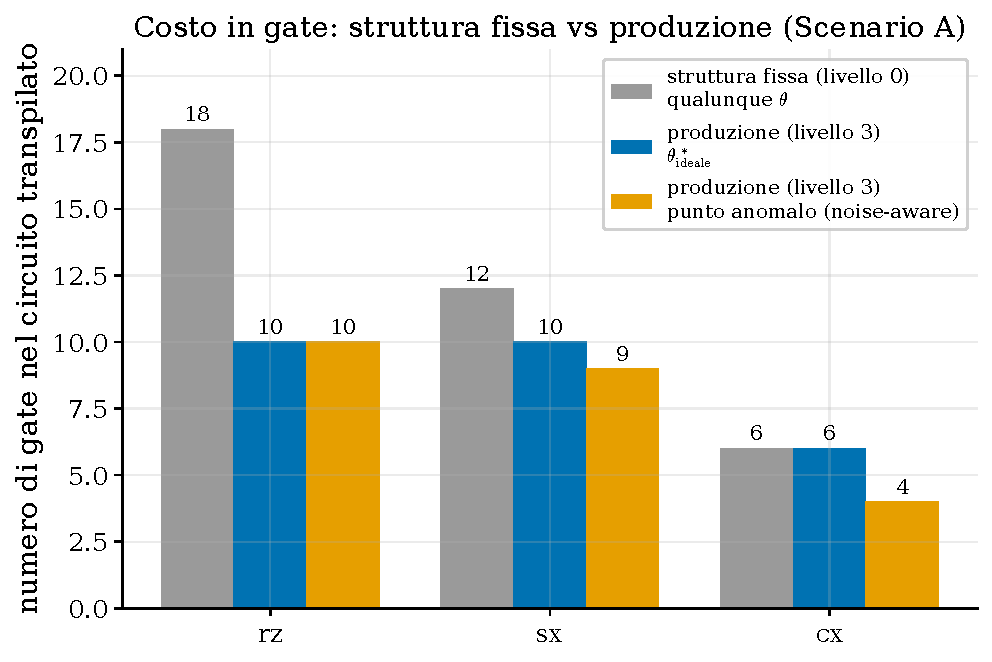
\includegraphics[width=0.75\textwidth]{figure/fig_bug_conteggio_gate_trimero_anello.pdf}
\caption{Costo in gate del circuito transpilato, Scenario A. A struttura fissa (livello 0) il
conteggio è sempre lo stesso, qualunque $\theta$. A produzione (livello 3), $\theta^*_\text{ideale}$
dà CNOT$=6$, ma un punto trovato dall'ottimizzatore noise-aware (vicino a $\theta_1{=}\pi$,
$\theta_2{=}0$) dà CNOT$=4$: il transpilatore semplifica il blocco CNOT--$R_y$--CNOT ai valori
speciali.}
\label{fig:bug-cnot}
\end{figure}

Su 5 assegnazioni casuali indipendenti, CNOT$=6$ sia a livello 3 sia a livello 0 --- il
comportamento anomalo non è generico, emerge solo quando l'ottimizzatore stesso trova valori
speciali di $\theta$ (Fig.~\ref{fig:bug-cnot}). A struttura fissa (livello 0), verificato che il
conteggio resta $6$ anche a quei valori speciali: la struttura fissa isola davvero l'effetto.

\verifica{Il punto anomalo trovato dal multistart noise-aware ha $\theta_1/\pi\approx0.99999637$,
$\theta_2/\pi\approx0.00889$ --- quasi esattamente $\pi$ e $0$. A questi valori il blocco
CNOT--$R_y(\theta)$--CNOT si semplifica e il transpilatore (livello 3) elimina 2 CNOT su 6.}

% =====================================================================
\section{Risultato 1: energia e fedeltà, a struttura fissa}
% =====================================================================

Multistart $R=12$ punti casuali $+\,1$ seme $=\theta^*_\text{ideale}$, a struttura fissa (livello 0).

\begin{table}[htbp]
\centering
\caption{Riuso ideale contro VQE noise-aware, struttura fissa (livello 0).}
\begin{tabular}{lccc}
\toprule
Quantità & Riuso $\theta^*_\text{ideale}$ & VQE noise-aware \\
\midrule
$E$ (rumoroso) & $-5.36232432$ & $-5.36648903$ \\
$F$ (rumorosa) & $0.96728547$ & $0.95153755$ \\
CNOT & 6 & 6 \\
\bottomrule
\end{tabular}
\end{table}

$\Delta E = -4.16\times10^{-3}$, $\Delta F = -1.57\times10^{-2}$ --- \textbf{energia migliore,
ma fedeltà peggiore}. Diverso, nella sostanza, dal dimero ($\Delta E\sim10^{-7}$, $\Delta F>0$):
qui la riottimizzazione sotto rumore trova genuinamente un punto diverso, non un rumore numerico
attorno allo stesso ottimo.

\messaggio{Il canale è isotropo su entrambi i sistemi, ma sull'anello (6 parametri, non 3) il
paesaggio ha evidentemente un punto stazionario dell'energia rumorosa misurabilmente distante da
$\theta^*_\text{ideale}$ --- l'argomento affine garantisce solo che $\theta^*_\text{ideale}$
resta un minimo di $E_\text{ideale}$, non che sia l'\emph{unico} minimo rilevante di
$E_\text{rumoroso}$ quando la dimensionalità cresce.}

% =====================================================================
\section{Robustezza del multistart: le due metodologie a confronto}
% =====================================================================

\begin{figure}[htbp]
\centering
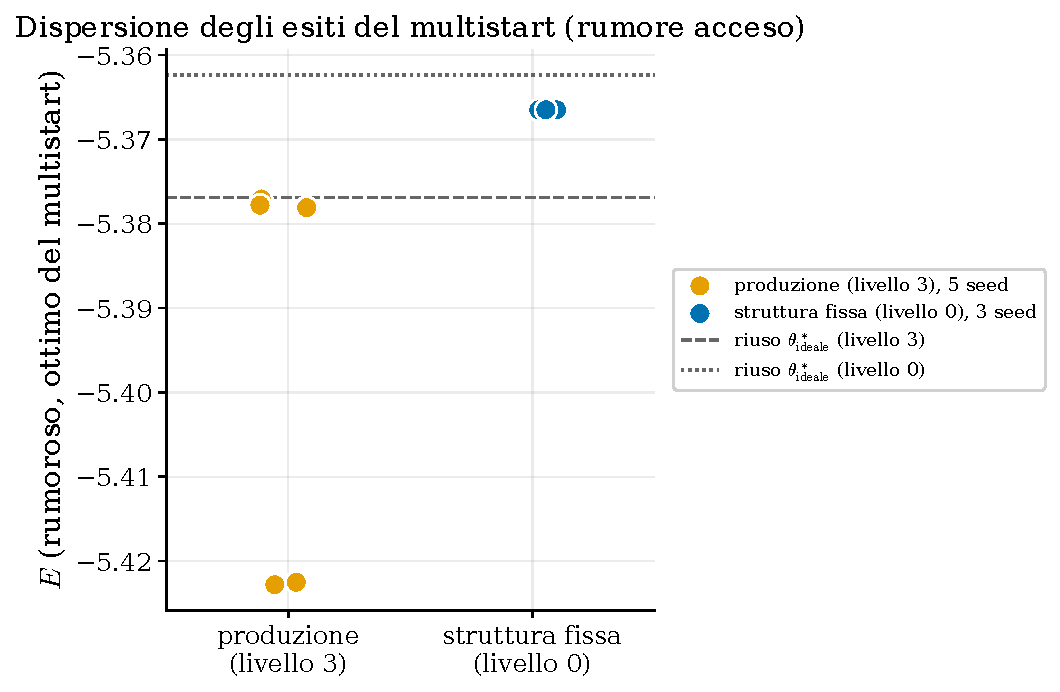
\includegraphics[width=0.78\textwidth]{figure/fig_robustezza_multistart_trimero_anello.pdf}
\caption{Dispersione degli esiti del multistart, 5 seed a livello 3 (produzione) contro 3 seed a
livello 0 (struttura fissa). A struttura fissa i tre punti sono sovrapposti (convergenza pulita);
a produzione i cinque seed si separano in due gruppi ben distinti.}
\label{fig:robustezza}
\end{figure}

\begin{table}[htbp]
\centering
\caption{Energia finale del multistart ($R=12+$seme), per seed, sulle due metodologie.}
\begin{tabular}{lccc}
\toprule
& $E$ & $\mathcal F$ & CNOT \\
\midrule
Struttura fissa, seed 0/1/2 & $-5.36648903$ (identico) & $0.951538$ & 6 \\
\midrule
Produzione, seed 0 & $-5.42250041$ & $0.963826$ & 4 \\
Produzione, seed 1 & $-5.42278742$ & $0.909939$ & 4 \\
Produzione, seed 2 & $-5.37706841$ & $0.699687$ & 4 \\
Produzione, seed 3 & $-5.37779324$ & $0.935748$ & 6 \\
Produzione, seed 4 & $-5.37808828$ & $0.962461$ & 6 \\
\bottomrule
\end{tabular}
\end{table}

A struttura fissa (Fig.~\ref{fig:robustezza}), 3/3 seed convergono identici entro $2\times10^{-11}$
--- paesaggio ben comportato, un solo ottimo rilevante. A produzione, dispersione di
$4.6\times10^{-2}$ in $E$ e fino a $0.26$ in $\mathcal F$: l'ottimizzatore trova, a seconda del
seed, punti con CNOT che oscilla fra 4 e 6 --- sta in parte esplorando artefatti del
transpilatore, non solo la fisica del problema. \textbf{Il risultato fisico di questo documento
si basa sulla versione a struttura fissa}; la versione a produzione è riportata come nota
metodologica a sé (\S8), non come risultato primario.

% =====================================================================
\section{Risultato 2: $N^*$ della fedeltà di Trotter}
% =====================================================================

\begin{figure}[htbp]
\centering
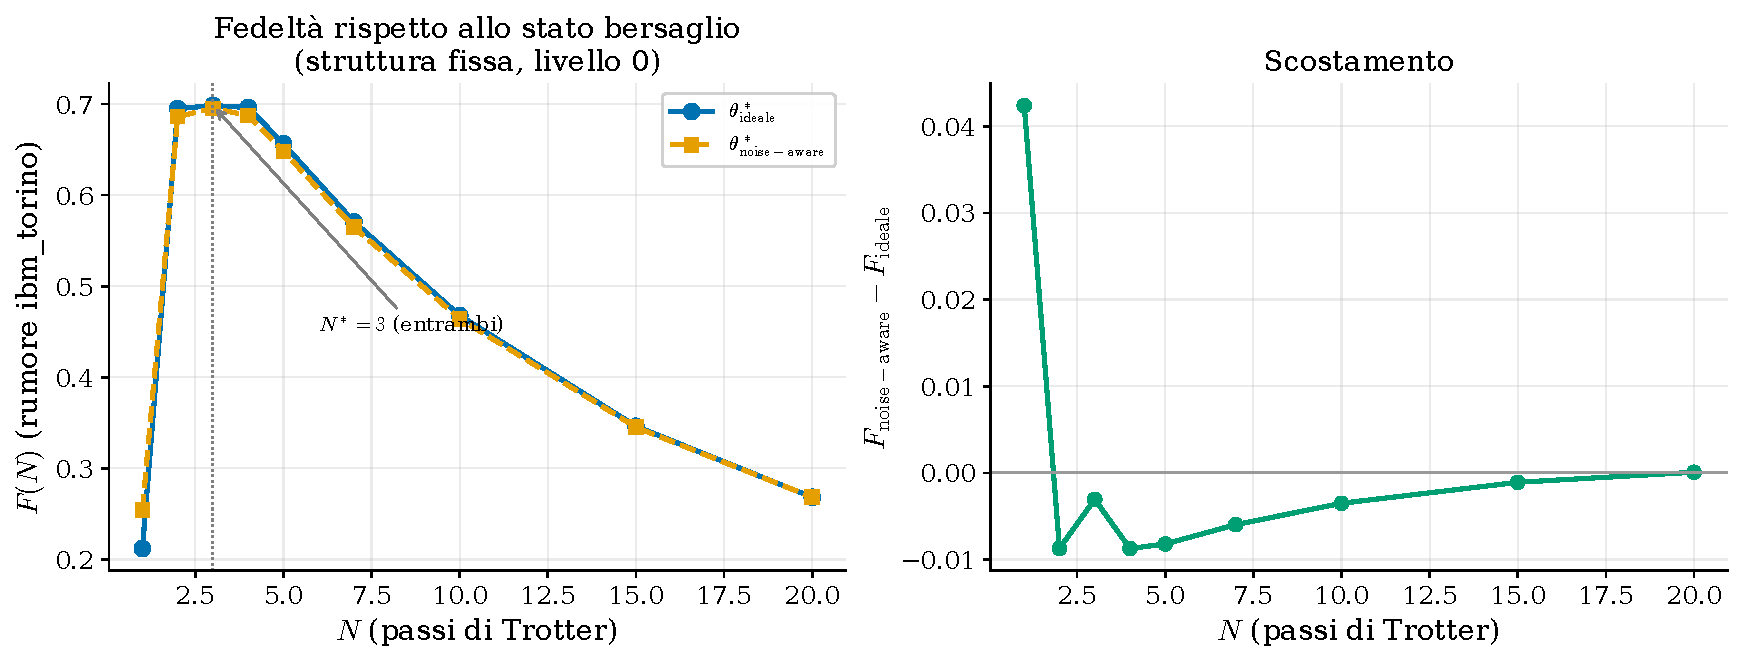
\includegraphics[width=\textwidth]{figure/fig_F_vs_N_confronto_trimero_anello.pdf}
\caption{Fedeltà $F(N)$ rispetto allo stato bersaglio, struttura fissa. \emph{Sinistra}: le due
preparazioni a confronto, $N^*=3$ in entrambi i casi. \emph{Destra}: scostamento, scala
$\sim10^{-2}$ --- un ordine di grandezza sopra il rumore numerico, ma piccolo rispetto alla scala
fisica del problema (la fedeltà stessa varia fra $0.2$ e $0.7$ sul range esplorato).}
\end{figure}

\begin{table}[htbp]
\centering
\caption{$N^*$ della fedeltà di Trotter, struttura fissa.}
\begin{tabular}{lcc}
\toprule
Preparazione & $N^*$ & $F(N^*)$ \\
\midrule
$\theta^*_\text{ideale}$ & 3 & 0.698381 \\
$\theta^*_\text{noise-aware}$ & 3 & 0.695324 \\
\bottomrule
\end{tabular}
\end{table}

$N^*=3$ invariato, coincide col baseline $N^*_A=3$ già noto dallo Stadio 3.

% =====================================================================
\section{Risultato 3: $N^*$ del correlatore dinamico}
% =====================================================================

\begin{figure}[htbp]
\centering
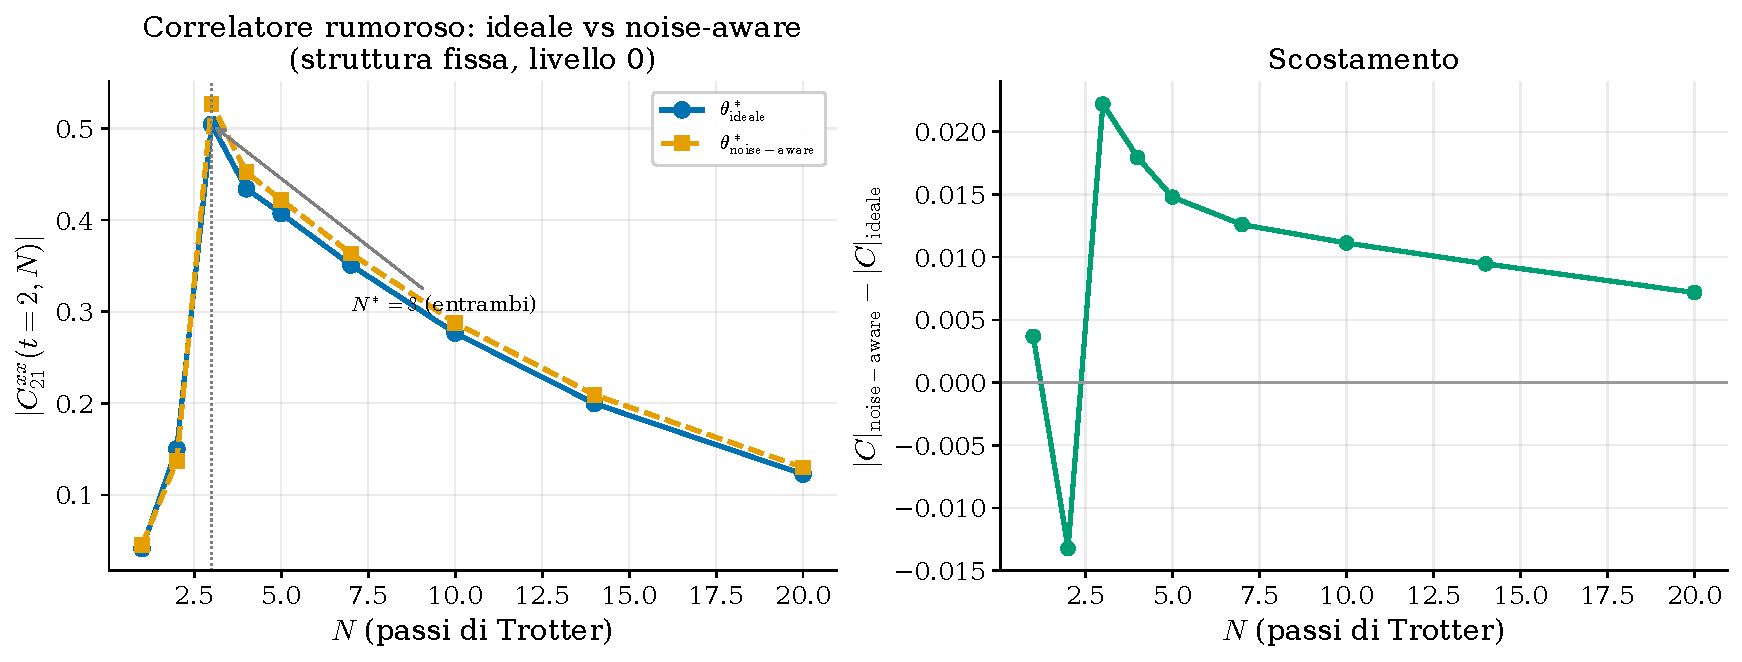
\includegraphics[width=\textwidth]{figure/fig_correlatore_noise_aware_confronto_trimero_anello.pdf}
\caption{Modulo del correlatore $|C_{21}^{xx}(t{=}2,N)|$, struttura fissa. $N^*=3$ in entrambi i
casi; lo scostamento (destra, scala $\sim10^{-2}$) ha segno misto in $N$, diverso dal
comportamento monotono osservato per la fedeltà di Trotter.}
\end{figure}

\begin{table}[htbp]
\centering
\caption{$N^*$ del correlatore dinamico, struttura fissa.}
\begin{tabular}{lcc}
\toprule
Preparazione & $N^*$ & $|C(N^*)|$ \\
\midrule
$\theta^*_\text{ideale}$ & 3 & 0.504443 \\
$\theta^*_\text{noise-aware}$ & 3 & 0.526657 \\
\bottomrule
\end{tabular}
\end{table}

$N^*=3$ invariato anche qui, coincide col baseline già noto (Stadio 4). Verificato
\textbf{direttamente}, non per analogia dal risultato precedente --- stessa disciplina già
motivata sul dimero (§2.1 del documento gemello): un conto valido per la fedeltà additiva non si
trasporta automaticamente al modulo di un correlatore.

% =====================================================================
\section{Nota metodologica: cosa succede a livello di produzione}
% =====================================================================

Per completezza, lo stesso controllo ripetuto sulla pipeline di produzione (livello 3), usando il
punto anomalo di Fig.~\ref{fig:bug-cnot} (seed 0, CNOT$=4$) al posto della versione a struttura
fissa.

\begin{figure}[htbp]
\centering
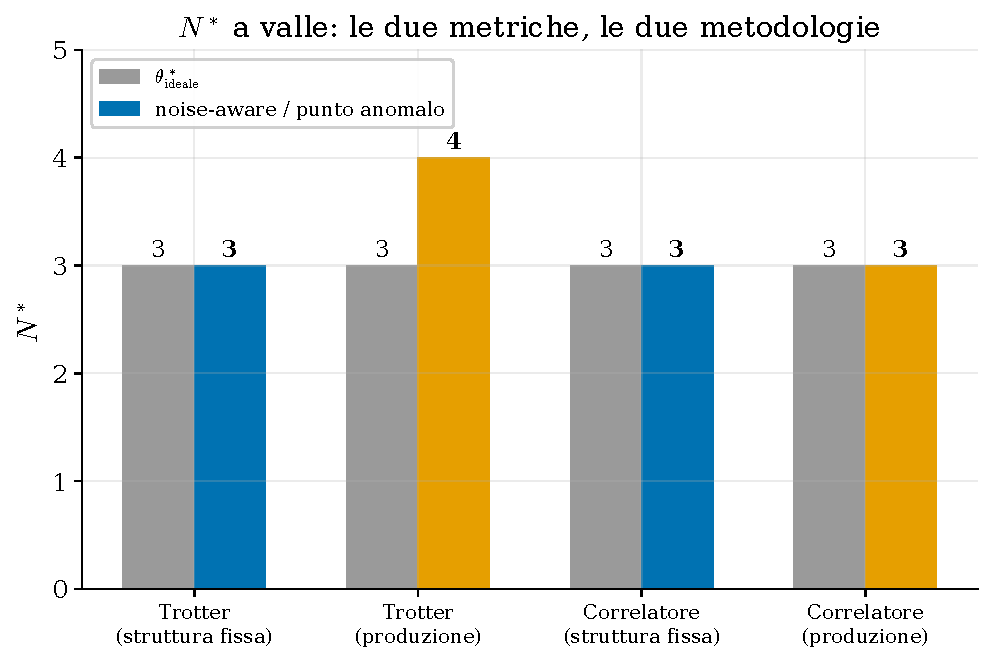
\includegraphics[width=0.72\textwidth]{figure/fig_Nstar_confronto_metodologie_trimero_anello.pdf}
\caption{$N^*$ a valle, le due metriche e le due metodologie a confronto. A struttura fissa,
invariato su entrambe. A produzione, il punto anomalo sposta $N^*$ per la fedeltà di Trotter
($3\to4$) ma non per il correlatore ($3\to3$).}
\label{fig:confronto-metodologie}
\end{figure}

\begin{table}[htbp]
\centering
\caption{$N^*$ a valle, produzione (livello 3), punto anomalo.}
\begin{tabular}{lcc}
\toprule
& $N^*$ Trotter & $N^*$ correlatore \\
\midrule
$\theta^*_\text{ideale}$ (livello 3) & 3 & 3 \\
Punto anomalo (livello 3) & \textbf{4} & 3 \\
\bottomrule
\end{tabular}
\end{table}

Un'asimmetria fra le due metriche mai osservata sul dimero (Fig.~\ref{fig:confronto-metodologie}):
il punto anomalo sposta $N^*$ per la fedeltà di Trotter (scarto piccolo: $F(3)=0.700335$ contro
$F(4)=0.693018$, ma il massimo cambia posizione) mentre lascia invariato $N^*$ del correlatore.
Non è un errore: è riproducibile (verificato in
\texttt{validate\_vqe\_noise\_aware\_trimero\_anello.py}, controlli 6--7), e riflette il fatto che
il punto anomalo non è uno stato ``vicino'' al fondamentale in senso generico --- è uno stato che
l'ottimizzatore ha trovato specificamente sfruttando una struttura di circuito diversa, quindi non
c'è motivo a priori che il suo effetto sulle due metriche a valle sia lo stesso.

\messaggio{Questa nota non invalida il risultato principale (§5--7, a struttura fissa): mostra
che la pipeline di produzione, se usata senza accorgimenti per un'estensione noise-aware su un
ansatz a più parametri, può restituire conclusioni dipendenti da un artefatto del transpilatore
--- una lezione metodologica utile per il seguito del progetto, non solo per questa estensione.}

% =====================================================================
\section{Perché l'argomento di continuità del dimero non si applica qui}
% =====================================================================

Sul dimero, l'invarianza di $N^*$ era spiegata da un argomento di continuità:
$\theta^*_\text{noise-aware}$ quasi indistinguibile da $\theta^*_\text{ideale}$
($\|\Delta\theta\|\sim10^{-4}$), quindi qualunque osservabile liscio a valle differisce di una
quantità altrettanto minuscola. \textbf{Qui $\|\Delta\theta\|$ non è piccolo}: a struttura fissa,
$\Delta E$ e $\Delta F$ sono tre ordini di grandezza più grandi del dimero, segno di uno
spostamento reale nello spazio dei parametri, non di un rumore numerico attorno allo stesso punto.
Che $N^*$ resti comunque invariato (§6--7) non è quindi spiegato dalla piccolezza di
$\Delta\theta$ (come sul dimero), ma da un fatto più debole e specifico di questo punto:
l'osservabile a valle è sufficientemente insensibile a \emph{questo particolare} $\Delta\theta$,
non ad un $\Delta\theta$ generico. Non generalizza automaticamente ad altri punti di lavoro o
altre soglie di rumore, a differenza del dimero dove l'argomento di continuità dava una garanzia
strutturale.

% =====================================================================
\section{Considerazioni}
% =====================================================================

\begin{itemize}
  \item \textbf{Il risultato principale è diverso da quello del dimero, non solo più complicato.}
  Sul dimero, riottimizzare sotto rumore non serve a nulla di misurabile. Sull'anello, a struttura
  fissa, produce un compromesso energia/fedeltà reale (energia migliore, fedeltà peggiore) --- ma
  questo compromesso non si traduce in uno spostamento di $N^*$ a valle, sulle metriche e al punto
  di lavoro testati.
  \item \textbf{La scelta metodologica (struttura fissa vs produzione) qui non è un dettaglio
  implementativo.} Sul dimero era irrilevante quale delle due si usasse (il conteggio gate era
  comunque invariante). Sull'anello, la scelta determina se si osserva un fenomeno fisico pulito
  o un artefatto del transpilatore mescolato alla fisica.
  \item \textbf{Il dominio di validità è più stretto che sul dimero}: un solo punto di lavoro
  (Scenario A), nessun argomento di continuità generale a sostegno. Un'estensione naturale (non
  fatta qui) sarebbe verificare se lo stesso quadro (energia migliore, fedeltà peggiore, $N^*$
  comunque invariato) si ripete a un secondo punto di lavoro VQE genuino sull'anello.
\end{itemize}

% =====================================================================
\section{Conclusioni}
% =====================================================================

Sul trimero ad anello, a differenza del dimero, riottimizzare l'ansatz \texttt{W-2q.6} sotto
rumore produce un effetto fisico misurabile: l'energia rumorosa migliora
($\Delta E=-4.16\times10^{-3}$) ma la fedeltà al vero stato fondamentale peggiora
($\Delta F=-1.57\times10^{-2}$) --- un compromesso mai osservato sul sistema a 2 spin. Nonostante
questo, $N^*$ resta invariato su entrambe le metriche a valle (fedeltà di Trotter, modulo del
correlatore), verificato a struttura di circuito fissa per isolare l'effetto fisico da un
artefatto del transpilatore specifico di questo ansatz a 6 parametri (CNOT che si riduce a valori
speciali di $\theta$, mai osservato sul dimero). Sulla pipeline di produzione, lo stesso artefatto
può spostare $N^*$ per una delle due metriche (Trotter) ma non per l'altra (correlatore) --- un
comportamento riproducibile, documentato come nota metodologica separata dal risultato fisico
principale.

\subsection*{Sintesi in una riga}
Sull'anello, a differenza del dimero, riottimizzare sotto rumore cambia lo stato trovato in modo
misurabile (energia meglio, fedeltà peggio) --- ma non sposta $N^*$ a valle, verificato isolando
l'effetto da un artefatto del transpilatore specifico di questo ansatz.

\subsection*{File prodotti}
\texttt{vqe\_noise\_aware\_\allowbreak trimero\_anello.py} (ottimizzazione, entrambe le
metodologie, Trotter e correlatore parametrici nel livello di transpilazione),
\texttt{validate\_vqe\_noise\_aware\_\allowbreak trimero\_anello.py} (8 controlli), questo
documento e le sue 5 figure. Aggiornamento in \texttt{log\_decisioni.md},
\texttt{scheda\_progetto\_tesi.md}.

\end{document}
